\chapter{Data Set}
\label{chapter:hps:dataset}

Proper search for \ac{dm} signals within the \ac{hps} detector includes both collection of data
with the \ac{hps} detector and simulation of how this apparatus responds to the physics of specific
processes. This chapter is focused on detailing the origin of these samples. The collected data can
be characterized by the known inputs from \ac{cebaf} and the run time. The simulation, as one might
expect, is a complicated multi-stage procedure in order to appropriately reflect the intricacies of
the real data.

\section{Collected Data} \label{sec:hps:data}
The data used in this study was collected over a series of 82 data collection runs within 2016
yielding a total of approximately one week of continuous beam.
The full luminosity of this data is estimated to be \qty{10.7}{pb^{-1}}.
As alluded to in \cref{sec:hps-ecal}, the collected data was triggered in order to focus the sample on
specific data of interest.

\subsection{Pair 1 Trigger} \label{sec:hps:data:trigger}
The trigger used for this and other physics analyses of the 2016 dataset is the so-called ``Pair 1 Trigger''
designed to select events where evidence for both an electron and positron have been found.
This trigger algorithm combines requirements on the energies of the clusters formed at the trigger
level along with the cluster locations.

After the hits in the \ac{ecal} are clustered, the clusters are selected such that they are of
high enough quality - implemented with energy $E$ and hit multiplicity $N$ cuts.
$$
  E_\mathrm{low} \leq E \leq E_\mathrm{high} \qquad N \geq N_\mathrm{min}
$$
With a beam energy of \qty{2.3}{\GeV}, we set $E_\mathrm{high}=\qty{1.4}{\GeV}$ to help remove
near-full-energy beam electrons from being included within this trigger.
$E_\mathrm{low} = \qty{0.15}{\GeV}$ and $N_\mathrm{min}=2$ are set to these values to suppress
the effect of noise.

All possible pairs of clusters passing these criteria where one of the pair is in the top half of
the \ac{ecal} and the other is in the bottom are then tested with further pair-wise criteria.
Let the top (bottom) cluster have energy $E_\mathrm{top}$ ($E_\mathrm{bot}$) and position
$(x_\mathrm{top},y_\mathrm{top})$ ($(x_\mathrm{bot},y_\mathrm{bot})$) leading to radius
$r_\mathrm{top} = \sqrt{x_\mathrm{top}^2+y_\mathrm{top}^2}$
($r_\mathrm{bot} = \sqrt{x_\mathrm{bot}^2+y_\mathrm{bot}^2}$).

The total energy of both clusters $E_\mathrm{top}+E_\mathrm{bot}$ is bounded below
by $E_\mathrm{sum,low}$ to remove noise and above by $E_\mathrm{sum,high}$ to reduce
the common single-bremsstrahlung background process.
The clusters are required to have an absolute difference $|E_\mathrm{top}-E_\mathrm{bot}| < E_\mathrm{diff}$
to select cluster pairs originating from the same particle.
The energy and position of the lower-energy cluster is required to satisfy
$E + r F \geq E_\mathrm{slope}$ which accounts for the expected bending of
the lower-energy particle's location in the magnetic field (which is failed
by clusters originating from photons which do not bend in the magnetic field).
$F$ is determined from the geometry of the detector and strength of magnetic
field to be $\qty{5.5}{\MeV\mm^{-1}}$.
Finally, the clusters are required to be coplanar within an angle $\phi$ to
again select for clusters originating from the same particle.
$$
  |\tan^{-1}(x_\mathrm{top}/y_\mathrm{top}) - \tan^{-1}(x_\mathrm{bot}/y_\mathrm{bot})| < \phi
$$

These requirements and the values selected for their thresholds are summarized
in \cref{tab:pair-1-trigger}.

\begin{table}[h]
  \centering
  \begin{tabular}{|r|c|c|}
    \hline
    Description & Variable & Value \\ \hline
    Single-Cluster Energy Minimum & $E_\mathrm{low}$ & \qty{0.15}{\GeV} \\
    Single-Cluster Energy Maximum & $E_\mathrm{high}$ & \qty{1.40}{\GeV} \\
    Single-Cluster Hit Count Minimum & $N_\mathrm{min}$ & 2 \\
    \hline
    Cluster Pair Energy Sum Minimum & $E_\mathrm{sum,low}$ & \qty{0.60}{\GeV} \\
    Cluster Pair Energy Sum Maximum & $E_\mathrm{sum,high}$ & \qty{2.00}{\GeV} \\
    Cluster Pair Energy Difference Maximum & $E_\mathrm{diff}$ & \qty{1.14}{\GeV} \\
    Low-Energy Cluster Slope Minimum & $E_\mathrm{slope}$ & \qty{0.70}{\GeV} \\
    Cluster Pair Azimuthal Difference Maximum & $\phi$ & \qty{35}{\degree} \\
    \hline
  \end{tabular}
  \caption{Values for cuts used within the Pair 1 Trigger during data collection of the HPS 2016 dataset.}
  \label{tab:pair-1-trigger}
\end{table}


\section{Simulation} \label{sec:hps:sim}
As mentioned the simulation goes through many steps in order to account for the different physics
processes that are of interest in a realistic fashion. In general, these steps are
\begin{enumerate}
  \item Generation -- using a tool like {\sc MadGraph/MadEvent}\todo[citation]{MG/ME citation} to generate
        specific events from Feynman diagrams
  \item Displacement -- if the sample expects to have the decay products be displaced (for example in the
        SIMP signal process), displace these decay products with a \emph{uniform} distribution of decay
        lengths to allow for re-weighting.
  \item Simulation -- simulate the detector response with \textsc{Geant4}\cite{geant4}
  \item Emulation -- emulate the readout electronics and triggering mechanism of collected data
\end{enumerate}
After this emulation stage, we can treat the simulation the same as the collected data,
applying the reconstruction and further analysis manipulatiuons and selections.

Moreover, simulated samples of standard data allows us to study how the detector responds in the
absence of such a signal process. These samples are produced in a similar way as iDM signal - just
with a different original generation step initializing the event (and inserting the physical
displacement distribution instead of a uniform one).

\section{Reconstruction}
\todo[lookup]{Brief overview of how events are reconstructed,
  especially with regard to tracks and vertices.}

\section{Analysis Pre-Selection}
The final stage that all events go through is a rudimentary pre-selection which simplifies the
resulting shape of the data in the event such that final analysis is not as complicated.
Specifically, the pre-selection for this analysis is requiring exactly one vertex to be
reconstructed within the event. This requirement naturally disposes of events which are cluttered
with particles from other beam arrivals (thus causing more than one vertex to be reconstructed) and
events which do not have a electron-positron pair within acceptance (thus causing no vertices to be
reconstructed). \cref{fig:n-vertex-pre-selection} shows the distribution of number of vertices
within an event for a variety of samples.

\begin{figure}
  \centering
  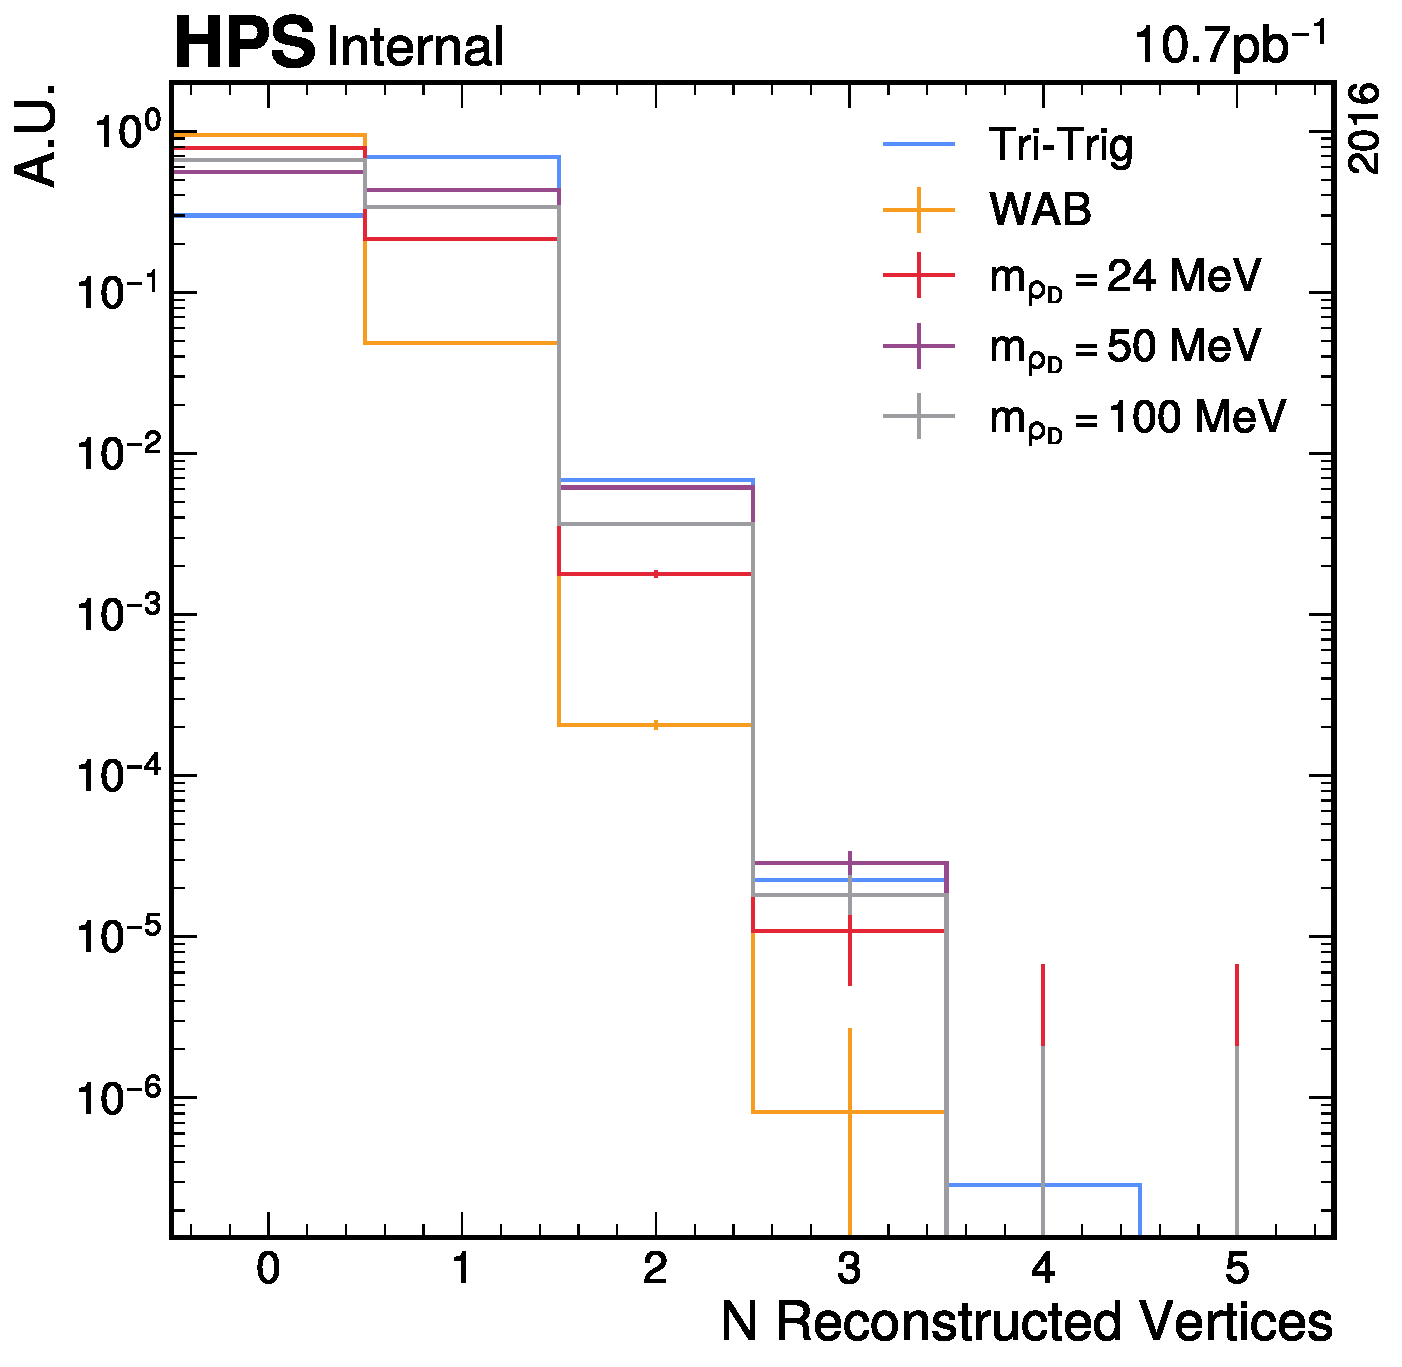
\includegraphics[width=0.5\textwidth]{figures/hps/dataset/n-vertex-pre-selection-mc-only.pdf}
  \caption{Number of vertices reconstructed within the simulation samples.}
  \label{fig:n-vertex-pre-selection}
\end{figure}
